\chapter{Literature Survey}\label{ch:literature_survey}
\epigraph{\textit{\Large “Adversarial training is the coolest thing since sliced bread”}}{\textit{ \large Yann LeCun,\\ Director of AI Research at Facebook \\and Professor at NYU}}
GANs were first introduced by Ian Goodfellow et al. in 2014[1] in Neural Information Processing Systems 2014 (NIPS 2014). The paper proposes a completely new framework for estimating generative models via an adversarial process. In this process two models are simultaneously trained. According to [1] the network has a generative model G that captures the data distribution, and a discriminative model D that estimates the probability that a sample came from the training data rather than G. This framework corresponds to a minimax two-player game. There is no need for any Markov chains or unrolled approximate inference networks during either training or generation of samples. This original work by Ian Goodfellow uses fully connected neural networks in the generator and the discriminator.\par\bigskip
\begin{figure}[H]
\centering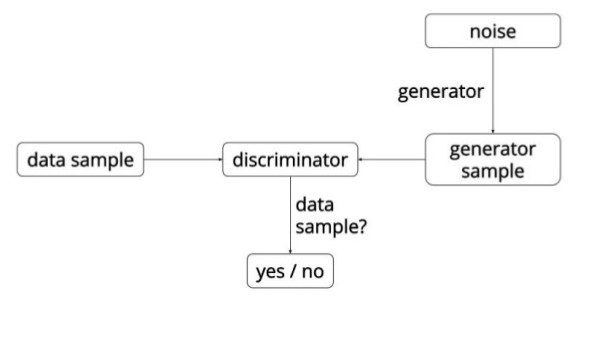
\includegraphics[width=.7\textwidth]{images/vanilaGAN.jpg}
\caption{Vanilla Generative Adversarial Network}
\end{figure}
Since then, there has been tremendous advancements in Deep Learning. A convolutional neural network (CNN, or ConvNet) [2] is a class of deep, feed-forward artificial neural networks that has successfully been applied to analyzing visual imagery. These networks uses convolution layers in its core. The convolution layer's parameters consist of a set of learnable filters, also called as kernels, which have a small receptive field, but they extend through the full depth of the input volume. During the forward pass, each filter is convolved across the width and height of the input volume, computing the dot product between the entries of the filter and the input and producing a 2-dimensional activation map of that filter. As a result, the network learns filters that activate when it detects some specific type of feature at some spatial position in the input.\par\bigskip
\begin{figure}[H]
\centering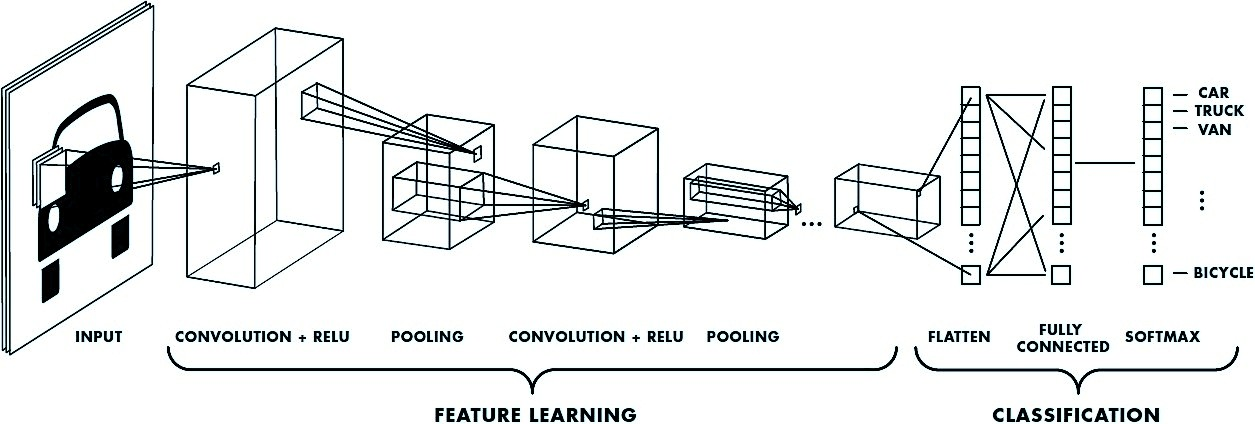
\includegraphics[width=.7\textwidth]{images/CNN.jpg}
\caption{Convolutional Neural Network}
\end{figure}
A breakthrough development that occurred in Adversarial Networks was the introduction of “Deep Convolutional Generative Adversarial Networks” by Alec Radford et al, ICLR, 2016 in 2016 in ICLR[3]. He applied a list of empirically validated tricks as the substitution of pooling and fully connected layers with convolutional layers.\par\bigskip
\begin{figure}[H]
\centering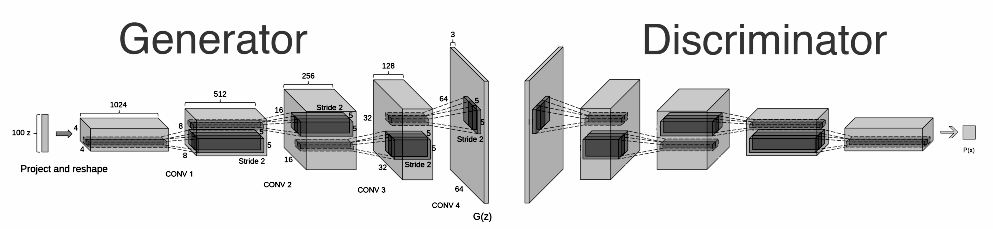
\includegraphics[width=1\textwidth]{images/dcgan.png}
\caption{Deep Convolutional Generative Adversarial Network}
\end{figure}
The power of the features encoded in the latent variables was further explored by Chen at al. [4]. They made use of the fact that the latent space of a regular GAN is underspecified to add additional input parameters (referred to as extend code) and thereby functionality. They decomposed the code in the latent code seen before and an additional latent component, which targets the semantic features of the data distribution. The goal is to learn disentangled and interpretable representations.\par\bigskip
Today, most GANs are loosely based on the former shown DCGAN [3] architecture. Many papers have focused on improving the setup to enhance stability and performance. Many key insights was given by Salimans et al.[5]:
\begin{itemize}
\item Usage of convolution with stride instead of pooling
\item Usage of Virtual Batch Normalization
\item Usage of Minibatch Discrimination in DD
\item Replacement of Stochastic Gradient Descent with Adam Optimizer [6]
\item Usage of one-sided label smoothing
\end{itemize}
Another huge development came with the introduction of Wasserstein GANs by Martin Arjovsky [7] . He introduced a new algorithm named WGAN, an alternative to traditional GAN training. In this new model, he showed that the stability of learning can be improved, remove problems like mode collapse, and provide good learning curves useful for debugging and hyperparameter searches.\par\bigskip
This recently proposed Wasserstein GAN (WGAN) makes progress toward stable training of GANs, but sometimes can still generate only low-quality images or fail to converge. 
Ishaan Gulrajani with Martin Arjovsky proposed an alternative in [8] to fix the issues the previous GAN faced. This proposed method performs better than standard WGAN and enables stable training of a wide variety of GAN architectures with almost no hyperparameter tuning, including 101-layer ResNets[9] and language models over discrete data.\par\bigskip
A big breakthrough in the field of Deep Learning came with the introduction of CapsNets or Capsule Networks[10] by the Godfather of Deep Learning, Geoffrey Hinton. CNNs perform exceptionally great when they are classifying images which are very close to the data set. If the images have rotation, tilt or any other different orientation then CNNs have poor performance. This problem was solved by adding different variations of the same image during training.\par\bigskip
\bigskip
\begin{figure}[H]
\centering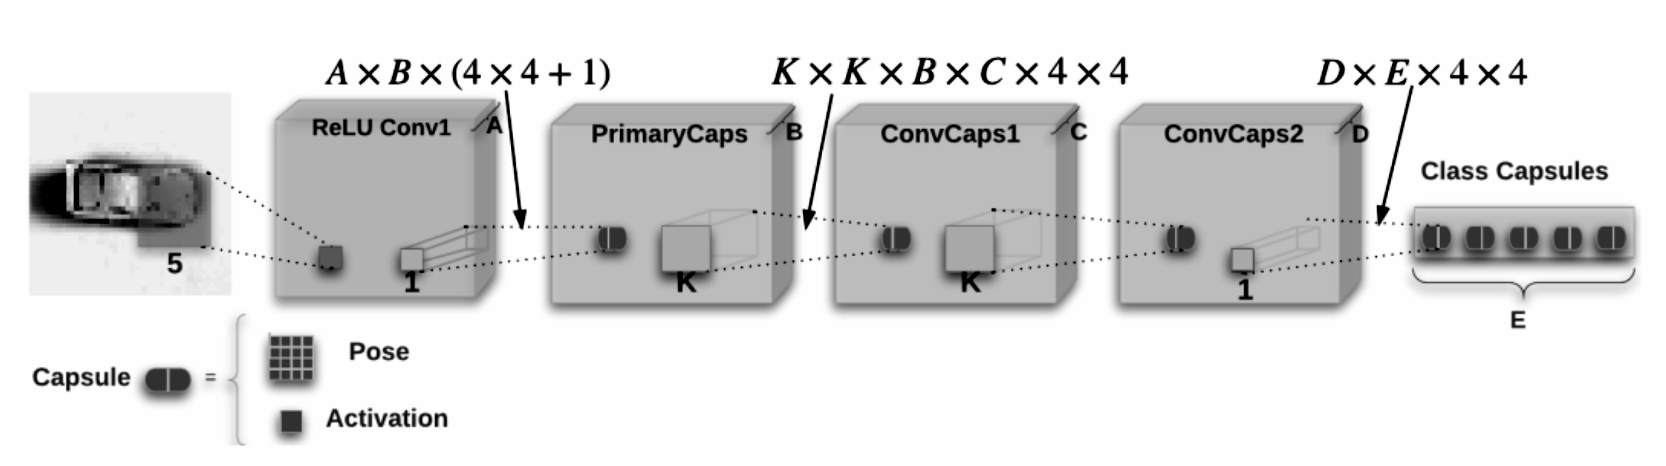
\includegraphics[width=1\textwidth]{images/caps.png}
\caption{Capsule Network}
\end{figure}
The key features of this breakthrough are Layer based Squashing and Dynamic Routing.
In a typical Convolutional Neural Network, the squashing function is added to each layer of the CNN model. A squashing function compresses the input to one of the ends of a small interval, introducing nonlinearity to the neural network and enables the network to be effective. Whereas, in a Capsule network, the squashing function is applied to the vector output of each capsule.\par\bigskip
Instead of applying non-linearity to each neuron, the squashing function applies squashing to a group of neurons i.e the capsule. To be more precise, it applies nonlinearity to the vector output of each capsule. The squashing function also tries to squash the vector output to zero if it is a small vector. If the vector is too long, the function tries to limit the output vector to 1.\par\bigskip
Dynamic routing algorithm in CapsNet replaces the scalar-output feature detectors of the CNN with the vector-output capsules. Also, the max pooling feature in CNNs, which led to positional invariance, is replaced with ‘routing by agreement’. The algorithm ensures that when they forward propagate the data, it goes to the next most relevant capsule in the layer above. Although dynamic routing adds an extra computational cost to the capsule network, it has been proved to be advantageous to the network by making it more scalable and adaptable.
